\chapter{Introduction}
\label{chap:intro}

Embedded systems are widely used today in various applications, from cars, cell phones, home automation, to critical infrastructures
like power plants and power grids, water, gas or electricity distribution systems and production systems for food and other products.
Within the context of an Industrial Control System (ICS), they are better known as PLCs (Programmable Logic Controllers).

Since they were almost isolated from the network, embedded systems have not been built with security in mind.
However, many recent cyber-attacks demonstrated that such an assumption is no more valid, and the security of embedded systems became an open question to deal with.

Unfortunately, this could be a more difficult long-term problem with respect to security for desktop and enterprise computing,
both for the limited capabilities of these systems and for the physical side effects a security breach may lead to, including property damage, personal injury, death and
even environmental or nuclear disaster.


\section{Problem statement}

The PLCs control the outside world via their I/O interfaces: therefore, they must be both reliable and secure.
Digging into their architecture, we know that the I/O interfaces of PLCs (e.g. GPIO, SCI, JTAG, etc.),
are usually controlled by a so called System on a Chip (SoC), an integrated circuit that combines multiple I/O interfaces.
In turn, the pins in a SoC are managed by a pin controller, a subsystem of SoC, through which one can configure the operating mode of the pins, such as the input or output mode.
One of the most peculiar aspects of a pin controller is that its behavior is determined by a set of registers: by altering these registers one can change the behavior
of the chip in a dramatic way. In \cite{ghostplc}, Abbasi et al. showed how this feature is exploitable by attackers, who can tamper with
the integrity or the availability of legitimate I/O operations, factually changing how a PLC interacts with the outside world.

Based on these observations, they introduced a novel attack technique against PLCs, called Pin Control Attack.
The salient features of this new class of attacks are:
\begin{enumerate}
	\item It is intrinsically stealth. The alteration of the pin configuration does not generate any interrupt, preventing the Operating System (OS) to react to it.
	\item It is entirely different in execution from traditional techniques such as manipulation of kernel structures or system call hooking, which are typically
		monitored by anti-rootkit protection systems.
	\item It is viable. It is possible to build concrete attack using it.
\end{enumerate}

To better understand a possible attack scenario, Fig. \ref{fig:control} shows a simplified control system.
\begin{figure}[h]
\centerline{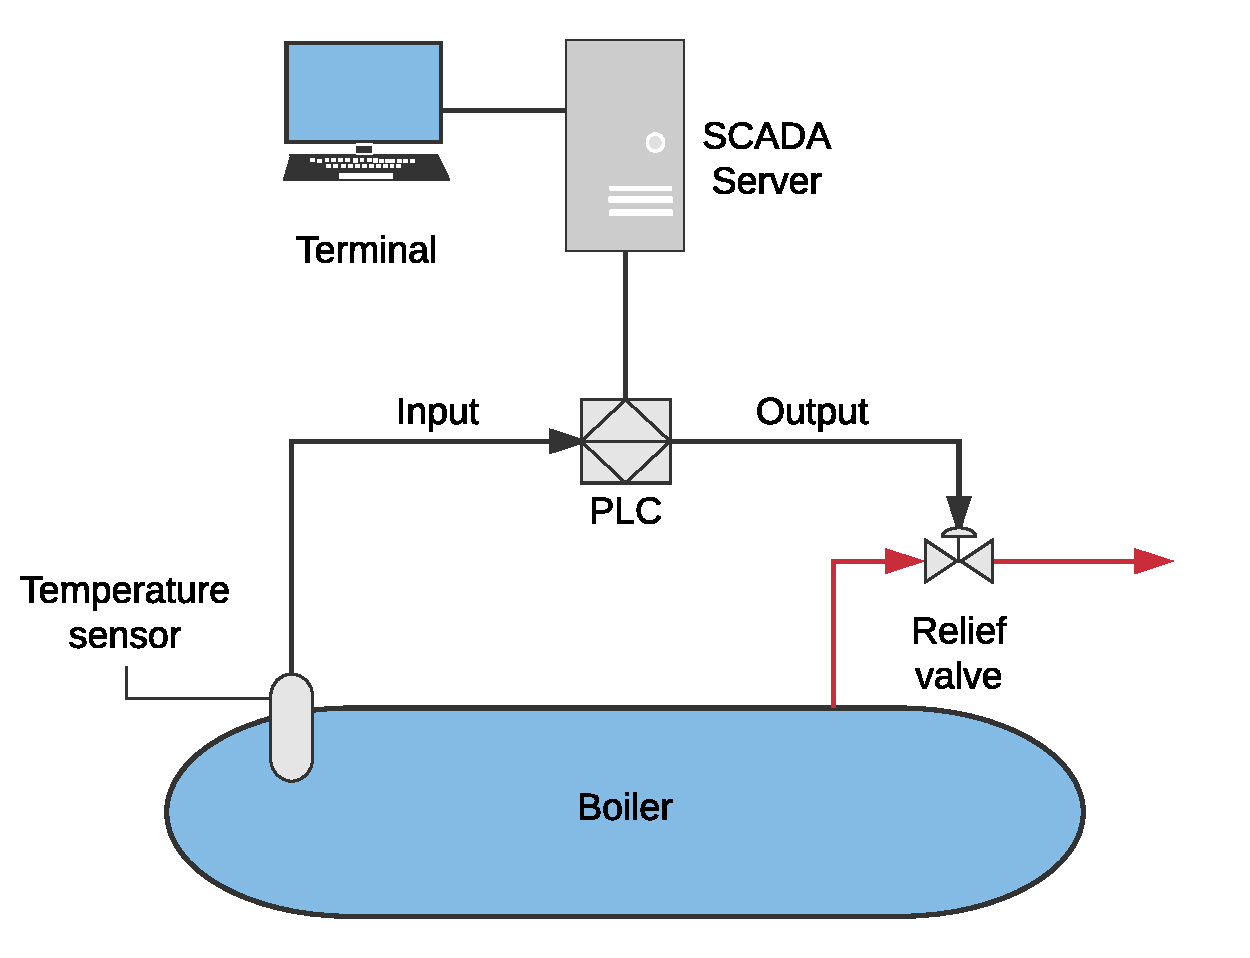
\includegraphics[width=0.6\textwidth]{res/control}}
\caption{Simplified control system: a possible target of Pin Control Attack.\label{fig:control}}
\end{figure}
The system consists of a boiler equipped with a relief valve driven by the PLC according to the value provided by a temperature sensor.
The PLC is connected to a SCADA server (Supervisory Control And Data Acquisition), which usually comes with a control software used to program the PLC itself
and to monitor its current status from a terminal.
Suppose that the PLC normally reads the values from the temperature sensor, and is programmed to open the relief valve if the temperature goes over $80^\circ C$.
An attacker could simply tamper the temperature value read by the PLC, reconfiguring the pin related to the sensor as output and writing its own desired value
(e.g. always $50^\circ C$) regardless of the actual temperature.
Actually there is no detection mechanism able to react to this configuration change, neither in the PLC firmware nor in the control system.
Moreover, the operator of the control system will not be able to see the real temperature from the terminal, but only the one forged by the attacker,
so it may likely not notice the intrusion at all.
Such a condition may lead to an uncontrolled overheating, and if it is not detected in time it could even make the boiler to explode.


\section{Aim of the thesis}

To overcome this sophisticated attack, we propose a defensive mechanism to extend the existing Linux Kernel Pin Control Subsystem, frequently used in embedded systems,
to be able to detect our novel attack. It is a challenging task for two reasons:
\begin{enumerate}
	\item The Pin Control lacks hardware interrupts, so it is not possible to directly react to any configuration change. More complex detection mechanisms are needed
		in order to achieve the highest possible detection rate.
	\item The resources available within an embedded system like a PLC are extremely limited. Therefore, our solution must be extremely agile and light
		since the smallest delay in the PLC I/O operation may have unintended consequences for the controlled process.
\end{enumerate}

Purpose of this thesis is to provide first a description of Pin Control Attack, discussing preconditions and effects.
Then, based on the obtained threat model, we want to describe and evaluate the design of a possible defense.
Finally, we provide an implementation for Linux Kernel on an ARM-based Programmable Logic Controller.
The implementation will be validated with respect to the following parameters: detection rate and performance overhead.
An organization of the thesis follows in the next section.


\section{Organization}

In \chap \ref{chap:related} we list the known attacks to embedded systems existing in the literature, and then discuss the protection mechanisms currently available.
As Pin Control Attack is a new kind of attack, to the best of our knowledge, at the time of writing, no one of the existing protections is able to prevent nor detect it.
In \chap \ref{chap:design} we present the architecture of our proposed Pin Control Protection, then we describe the implementation and provide developer and user manual for it.
The \chap \ref{chap:results} provides the results obtained during the experiments, showing the detection rate and the performance overhead on a PLC environment.
Finally, in \chap \ref{chap:conclusions} we analyse the shortcomings of our defense and the possible future works and improvements.
